%!TEX root=../document.tex

\section{Einführung}
Installieren und Konfigurieren Sie eine NAS Appliance welche Block Devices (Festplatten) über iSCSI im Netzwerk freigeben kann (z.B. openfiler1, FreeNAS) falls diese nicht bereits für die Übung zur Verfügung gestellt wurde (je nach Gruppe/Zeitplan).

\subsection{Ziele}


\begin{itemize}
	\item Das iSCSI Target soll automatisch beim booten des Clients/Initiators verbunden werden
	\item Installieren Sie ocfs2 auf mindestens 3 Computern (die auf das Block-Devices per iSCSI verbunden sind)
	\item Konfigurieren Sie einen OCFS2 Cluster für diese 3 Computer (Nodes), z.B. über die Datei /etc/ocfs2/cluster.conf
	\item Formatieren Sie das gemeinsame iSCSI Block Device im OCFS2 Dateisystem (mkfs.ocfs2) - dies muss nur auf einem Computer durchgeführt werden, da es sich ja um ein Cluster-Dateisystem handelt
	\item Überprüfen Sie, wie sich das Dateisystem bei gemeinsamen Zugriff auf eine Datei verhält
	\item Dokumentieren Sie Ihre Durchführung Ihre Ergebnisse
\end{itemize}
Die Arbeit ist in Gruppen zu 3-4 Teilnehmern möglich. Jeder Teilnehmer muss den iSCSI-Initiator und OCFS2 konfiguriert haben

Abgabe des Protokolls (1x/Gruppe) als pdf.

\subsection{Voraussetzungen}
Welche Informationen sind notwendig um die Laborübung reibungslos durchführen zu können? Hier werden alle Requirements der Lehrkraft detailliert beschrieben und mit Quellen untermauert.

Hier zum Beispiel die Architektur der \textit{Common Object-Request-Broker Architecture}:
\begin{figure}[!h]
	\begin{center}
		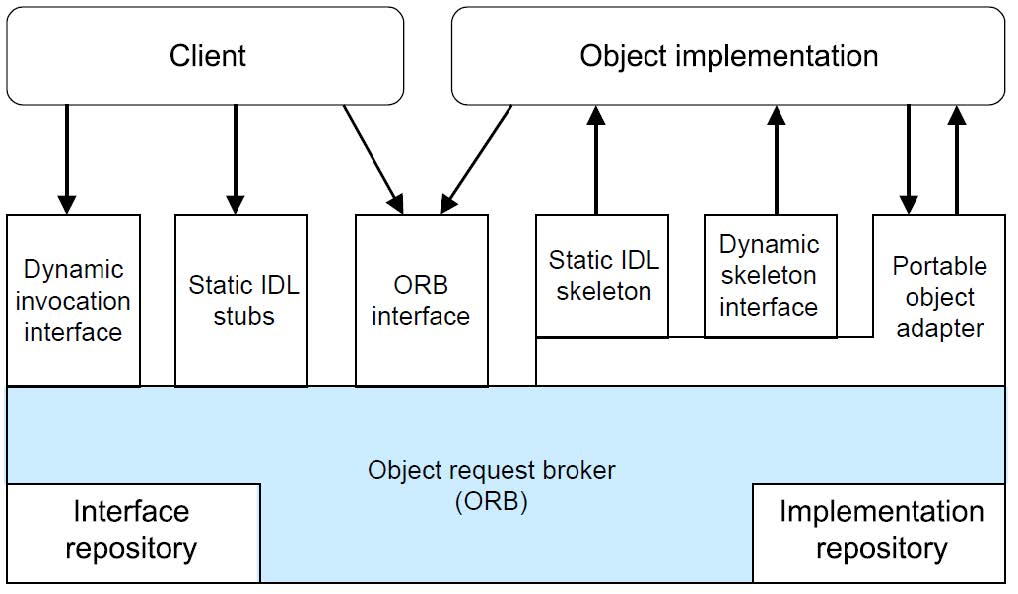
\includegraphics[width=0.5\linewidth]{images/corba.jpg}
		\caption{Common Object-Request-Broker Architecture \cite{tanenbaum2007verteilte}}
		\label{broker}
	\end{center}
\end{figure}


\subsection{Aufgabenstellung}
Hier wird dann die konkrete Aufgabenstellung der Laborübung definiert.

Nun kommt ein Seitenumbruch, um eine klare Trennung der Schülerarbeit zu bestimmen.
\clearpage
